This section presents two forms of evaluations of our gaze model. The first evaluation involved an \textit{objective} assessment of the effectiveness of our model in reducing the frequency and severity of visual artifacts in gaze shifts on different character designs. The second evaluation followed a human-subjects study and assessed the \textit{perceived} characteristics of the generated gaze behaviors.

\subsection{Objective Evaluation}

To evaluate the effectiveness of our model in reducing visual artifacts, we have conducted measurements of artifact prevalence on a variety of characters using a set of objective metrics. These metrics reflected the amount of observable artifacts over the course of a gaze shift. Because each artifact is a product of a particular combination of the pose and movement of the eyes and the head, whether or not the artifact is present at a particular frame and its severity can be objectively determined and quantified. Each metric computes the presence of an artifact in each frame and sums them over all the frames of the gaze shift to calculate the ``amount'' in which the artifact appears. Severity is determined by weighing the amount of an artifact by the cosine fall-off of the viewing angle, $\phi$ (i.e., angle between view direction and character's gaze direction), thus giving less weight to frames where the character's eyes are less visible. The artifact amount is also weighed by the blink height at each frame to account for eye blinks that partially or fully conceal artifacts. The aggregated amounts are then normalized by the duration of the gaze shift, providing us with quantities that we can compare across different characters and gaze shift configurations. Our metrics include cross-eyedness amount, $\tau_{CE}$, OMR-block amount, $\tau_{OMR}$, eye retraction and divergence amount, $\tau_{ERD}$, and stuck eye amount, $\tau_{SE}$.
% NOTE: removed redundant explanations of metrics -- Tomislav

% See http://www.inf.ethz.ch/personal/markusp/teaching/guides/guide-tables.pdf for info on making nice tables
\begin{table}[b!]
\footnotesize
\centering
\caption{Quantitative evaluation results. Each cell contains the aggregate score for a particular metric on a particular character with the baseline model or our proposed model.}
\vspace{4pt}
\begin{tabular}{@{}llcccc@{}}\toprule
Character & Model & $\tau_{CE}$ & $\tau_{OMR}$ & $\tau_{ERD}$ & $\tau_{SE}$ \\
\midrule
RealisticFemale1 & \textbf{Baseline} & 0.30 & 0.24 & 0.20 & 0.03 \\\hdashline
RealisticFemale2 & \textbf{Baseline} & 0.31 & 0.22 & 0.20 & 0.03 \\\hdashline
\multirow{2}{*}{SemiStylizedFemale} & \textbf{Baseline} & 0.31 & 0.23 & 0.18 & 0.03 \\
& \textbf{Proposed} & 0.07 & 0.10 & 0.10 & 0.02 \\\hdashline
\multirow{2}{*}{StylizedFemale} & \textbf{Baseline} & 0.40 & 0.25 & 0.21 & 0.05 \\
& \textbf{Proposed} & 0.12 & 0.10 & 0.10 & 0.02 \\\hdashline
\multirow{2}{*}{StylizedMale} & \textbf{Baseline} & 0.32 & 0.22 & 0.17 & 0.03 \\
& \textbf{Proposed} & 0.09 & 0.10 & 0.10 & 0.03 \\\hdashline
\multirow{2}{*}{EmotiGuy} & \textbf{Baseline} & 0.27 & 0.33 & 0.20 & 0.07 \\
& \textbf{Proposed} & 0.06 & 0.12 & 0.13 & 0.03 \\\hdashline
\multirow{2}{*}{Jack} & \textbf{Baseline} & 0.06 & 0.46 & 0.11 & 0.05 \\
& \textbf{Proposed} & 0.07 & 0.16 & 0.07 & 0.06 \\\hdashline
\multirow{2}{*}{Donkey} & \textbf{Baseline} & 0.18 & 0.34 & 0.22 & 0.10 \\
& \textbf{Proposed} & 0.04 & 0.10 & 0.15 & 0.03 \\\hdashline
\multirow{2}{*}{Fish} & \textbf{Baseline} & 0.54 & 0.30 & 0.26 & 0.08 \\
& \textbf{Proposed} & 0.16 & 0.10 & 0.14 & 0.03 \\\hdashline
\multirow{2}{*}{NastyMonster} & \textbf{Baseline} & 0 & 0.20 & 0.29 & 0 \\
& \textbf{Proposed} & 0 & 0.09 & 0.18 & 0 \\
\bottomrule
\end{tabular}
\label{tab:EvalResults}
\end{table}

For our test cases, we generated $138$ random gaze shifts and applied them to ten different characters, including two with realistic, humanlike proportions (Figure~\ref{fig:TestCases}). The gaze shifts included an even number of shifts with full and minimal head alignment. For each character, we aggregated the measurements for all gaze shifts with the same head alignment. The results show a reduction in artifact prevalence in almost all test cases as summarized in Table~\ref{tab:EvalResults} and below:

\begin{itemize}

\item Cross-eyedness, $\tau_{CE}$, in characters with human proportions has an average value of $0.30$ and goes up to $0.54$ in characters with larger inter-eye distances. These levels of cross-eyedness cause unacceptable visual artifacts in stylized characters with large eyes, which are significantly reduced by our model.

\item $\tau_{OMR}$ is $0.22$--$0.24$ for realistic characters and can be as high as $0.46$ in stylized characters with very narrow OMR such as Jack. Our model reduces it by $30$--$60$\%, bringing it to about half of normal human levels and achieving a slower movement toward OMR in larger eyes.

\item $\tau_{ERD}$ is approximately $0.20$, $0.30$, and $0.10$ in realistic characters, characters with wide (e.g., NastyMonster) or highly asymmetric OMR (e.g., Fish), and characters with low OMR (e.g., Jack), respectively. Our model succeeds in reducing these values by $30$--$50$\%.

\item Even characters with human proportions exhibit a small amount of stuck eye, $\tau_{SE}$, which we believe is too small to notice. With characters with asymmetric OMR (e.g., EmotiGuy, Jack, Donkey, Fish), $\tau_{SE}$ can be as high as $0.10$. Our model reduces it to levels seen in human characters. An exception is the Jack character with very narrow OMR, which offers little flexibility in the movement.

\end{itemize}

\subsection{Human Subjects Study}

To lessen visual artifacts and afford staging effects, our model deliberately directs the characters's gaze shifts toward locations that are different from the intended gaze targets. While these shifts do not involve geometrically accurate gaze motions, previous studies on gaze perception have shown that people are generally imprecise at judging gaze direction \cite{argyle1976gaze}, suggesting that these deviations might not worsen judgments that already show very high variability. Therefore, the evaluation sought to determine whether these deviations affected the communicative accuracy and perceived naturalness of gaze shifts generated by our model compared with a previously validated baseline model \cite{andrist2012headeye}.

% TODO: Any information on participant profile?
\textit{Participants} -- We recruited 48 participants using the Amazon Mechanical Turk crowd-sourcing service. Each participant was paid U.S. \$1 for their participation.

\textit{Study Design} -- The study followed a three-by-one, between-participants design. The experimental conditions included gaze shifts performed by (1) \textit{baseline}: a character with human proportions following the baseline gaze model, (2) \textit{baseline stylized}: a character with stylized geometry following the baseline gaze model, and (3) \textit{stylized}: a character with stylized geometry following our gaze model. We chose a between-participants design to minimize transfer effects. Figure~\ref{fig:StudyTask} illustrates the two characters used in the study. The \textit{stylized} condition involved performative gaze shifts with an eye-alignment parameter of $0.85$.

\begin{figure}[t]
\centering
\includegraphics[width=0.48\textwidth]{Figures/StudyTask-small.pdf}
\caption{Stills from videos in our study. Left: Realistically-proportioned character. Right: Stylized character.}
\vspace{-12pt}
\label{fig:StudyTask}
\end{figure}

\textit{Task} -- Participants in the study watched a series of videos of the character shifting its gaze toward numbered targets arranged on a whiteboard and tried to identify the target toward which the character was looking (Figure~\ref{fig:StudyTask}). The character was positioned in front of the camera, approximately $1 m$/$3.3 ft$ away and slightly to the right. The whiteboard was positioned on the character's right and oriented so that the viewer and the character could comfortably see the targets.

\textit{Procedure} -- After recruitment, each participant reviewed and agreed to a consent form. Following informed consent, the participants viewed a sequence of $22$ videos. In each video, the character shifted its gaze toward a randomly selected target from among nine targets on the whiteboard. After watching each video, the participants were asked to determine the target toward which the character was looking and provide their answer in a text field. Each video was approximately ten seconds in length. At the beginning of each video, the character looked toward the camera and nodded. It then shifted its gaze toward one of the targets, maintained its gaze at the target for two seconds, and then looked back toward the viewer.

To ensure the quality of the experimental data, we followed crowd-sourcing best practices \cite{kittur2008mturk}. For example, all participants were shown two training and acclimation videos, where    the correct gaze target would light up during the gaze shift. Data from participants who failed to correctly identify the target were discarded. We also restricted the task to workers with high approval rates and tracked statistics such as task completion time and screen resolution.
% NOTE: Explained our quality control procedure in more detail. -- Tomislav

At the end of the study, each participant filled out a questionnaire to provide subjective evaluations of the character. The study took approximately ten minutes.

\begin{figure}[!b]
\centering
\vspace{-8pt}
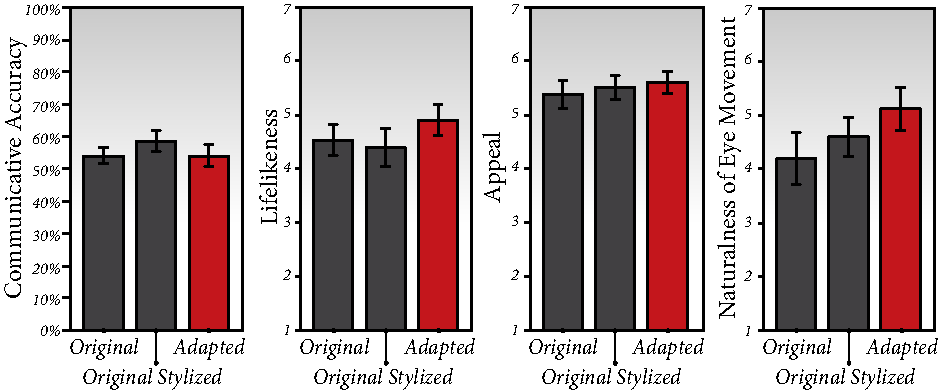
\includegraphics[width=0.48\textwidth]{Figures/Results.pdf}
\caption{Results for communicative accuracy, lifelikeness, appeal, and naturalness of eye movements. Data on gaze shifts generated by our model are shown in red.}
\vspace{-8pt}
\label{fig:StudyResults}
\end{figure}

\textit{Measurement \& Analysis} -- The dependent variables in our study were \textit{communicative accuracy}, \textit{naturalness of eye movements}, \textit{lifelikeness}, and \textit{appeal}. Communicative accuracy was measured as the percentage of correctly identified gaze targets. Naturalness of eye movements, lifelikeness, and appeal were measured using a questionnaire. Participants rated each item in the questionnaire using seven-point rating scales ($1 = not likable$; $7 = likable$). The lifelikeness scale included three items that measured lifelikeness, humanlikeness, and believability ($Cronbach's \alpha = 0.799$), while the appeal scale included four items that measured charisma, attractiveness, cuteness, and likability ($Cronbach's \alpha = .796$).

Data analysis included one-way analysis of variance (ANOVA) tests, following guidelines suggested by Julnes and Mohr \cite{julnes1989analysis} for establishing a ``no difference'' in comparisons, particularly an alpha level of $0.25$ (i.e., $p > .25$) to control for Type II errors.
%http://deepblue.lib.umich.edu/bitstream/2027.42/67182/2/10.1177_0193841X8901300604.pdf

\textit{Results} -- Results for all measures are illustrated in Figure \ref{fig:StudyResults}. The mean accuracies in the baseline, baseline stylized, and stylized conditions were $54.0\%$, $58.6\%$, and $54.0\%$, respectively. The statistical analysis of the data found no significant effect of our manipulation on accuracy, $F(2,45) = 0.83$, $p = 0.44$. These rates are considerably better than chance, which we expect to be closer to 1/3 than 1/9, as our informal analysis suggests that it is easy to determine toward which row is being looked, and are consistent with results from previous work \cite{argyle1976gaze,goldberg1969distance,andrist2012designing}. Pairwise contrast tests also found no differences between the baseline and baseline stylized conditions, $F(1,45) = 0.00$, $p = 1.00$, or between the baseline and stylized conditions, $F(1,45) = 1.20$, $p = 0.28$. These results suggest that our model retains the communicative accuracy of the baseline human model.

Our analysis revealed no significant effect of our manipulation on naturalness of eye movements, $F(2,45) = 1.27$, $p = 0.29$. Contrast tests also found no differences between the baseline and baseline stylized conditions, $F(1,45) = 0.53$, $p = 0.47$, or between the baseline and stylized conditions, $F(1,45) = 2.52$, $p = 0.12$, suggesting that our model preserves the naturalness of eye movements generated by the baseline model.

We found no significant effects of our manipulation on the lifelikeness measure, $F(2,45) = 0.69$, $p = 0.51$. Pairwise contrasts showed no differences between the baseline and baseline stylized conditions, $F(1,45) = 0.10$, $p = 0.75$, or baseline stylized and stylized conditions, $F(1,45) = 0.64$, $p = 0.43$. Similarly, we found no effects of our manipulation on the appeal measure, $F(2,45) = 0.25$, $p = 0.78$. No differences appeared in pairwise contrast tests between the baseline and baseline stylized conditions, $F(1,45) = 0.18$, $p = 0.68$, or baseline stylized and stylized conditions, $F(1,45) = 0.49$, $p = 0.49$.

Overall, the results suggest that our gaze model does not change the communicative accuracy and the subjective evaluation of the characters. While we speculate that the removal of artifacts may improve a character's appeal, such effects are unlikely to appear in short, focused tasks. Future studies might further explore how our model shapes subjective impressions of the character in longer, more realistic scenarios.